\chapter{Directly Interacting with Memory Content}\label{chp:casting}
\epigraph{When I see a bird that walks like a duck and swims like a duck and quacks like a duck, I call that bird a duck.}{James Whitcomb Riley}

In the previous chapter we've seen how we can use C to perform simple computations. The inputs for these computations were given \emph{at compiletime}. That means, once the program was compiled, it would always churn out the same result; we could not reuse the compiled executable to get new results, but always had to edit the code and recompile. In this chapter, we'll use our knowledge about pointers and memory structure to write \emph{interactive} code: programs that take some input from the user \emph{at runtime}, \ie values that were not determined when the code was written. While we're at that, we will also discuss some \enquote{bit magic}, \ie operations that directly take the bitpatterns of the information in memory into account.

\section{Reading Values with \texttt{scanf}}
The command \texttt{scanf} instructs the computer to let the user type some text on the keyboard, interpret it one or another way (\eg as integer or floating point number) and then store it in memory. Unfortunately, we can't instruct the CPU \emph{directly} to store information in a variable. This is because, for the CPU there are no variables -- only memory addresses. Variables are names we give to memory addresses to make life for us humans easier. The compiler knows which variable name belongs to which memory address, but after it has done its job, there are no names left in the compiled machine code -- only numbers. The command \texttt{scanf} invokes such machine code and is therefore incompatible with human language variable names. To do its job (writing a number to memory), we need to provide the \emph{address} of the variable that should store the number.

We are by now very familiar with the fact that the same information can be interpreted in different ways. In the previous chapter, when we learned about \texttt{printf}, we were concerned with the converision rules from binary (information in memroy) to text (information on screen). In a way, \texttt{scanf} is the counterpart to \texttt{printf}: it takes text information from the user and converts it into a bitpattern. With this preface, you will not be surprised to hear that the format strings we already know about make a comeback\footnote{Also maybe you remember that the \texttt{f} in \texttt{printf} stands for \emph{formatted}. It means the same in \texttt{scanf}.}.

\subsection{Simple Usage}
The simplest way to use the command is the following:

\begin{codebox}[Syntax: \texttt{scanf}]
scanf(formatString, pointerToVariable)
\end{codebox}
in which, again:
\begin{itemize}
\setlength\itemsep{0pt}
\item \texttt{formatString} is text comprising of format codes like \texttt{\%d} which tells how to interpret the user input.
\item \texttt{pointerToVariable} is the address of a variable which should be overwritten with the interpreted user input.
\end{itemize}

Let's look at an example and go through it line by line:
\begin{codebox}[interactiveSum.c]
\begin{minted}[linenos]{c}
#include <stdio.h>

int main () {
    int first = 0, second = 0;
    
    printf("Please enter a first number: ");
    scanf("%d", &first);
    printf("Please enter a second number: ");
    scanf("%d", &second);
    
    printf("The sum of the two is %d\n", first + second);
}
\end{minted}
\captionof{code}{Using \texttt{scanf} to read values from the keyboard} \label{code:scanfSimple}
\end{codebox}
\begin{itemize}
\setlength\itemsep{0pt}
\item Line 1 is of course the well known \texttt{include} directive. We knew before that this command allows us to use the \texttt{printf} command; 
	we also get the \texttt{scanf} command from this directive.
\item In line 4 we declare two integer variables and set them to zero.
\item Line 6 prompts the user to enter a number. Note how the format string \emph{does not} end in \texttt{\textbackslash n} here; 
	the cursor remains in the same line as the text just written.
\item The \texttt{scanf} command begins by waiting for user input. Whatever the user may type will appear on screen (directly after \texttt{... first number:}).
	When the user is done entering values (\ie when they hit the \emph{return} key), it will attempt to interpret the input according to the format string.
	The format string is \texttt{"\%d"}, which signifies an integer. If the user input could be interpreted as an integer (the user may also enter \texttt{banana}, 
	which cannot be converted into a number\citationneeded[https://xkcd.com/2070/]), this interpretation is written \emph{to the address} \texttt{\&a}.
\item Lines 8 and 9 repeat the above wiht \texttt{\&b}
\item After this, we can use the previously read values which are now stored in the variables \texttt{a} and \texttt{b} to do regular computations like that in line 11.
\end{itemize}

Consequently, running this code could produce output like this:
\begin{cmdbox}[Possible output: interactiveSum.c]
Please enter a first number: 3 \\
Please enter a second number: 4 \\
The sum of the two is 7
\end{cmdbox}


\begin{plusbox}[Why does \texttt{printf} need no addresses?]
Both, the instructions behind the commands \texttt{printf} and behind \texttt{scanf} are available as compiled code, \ie in machine language. As we've learned before, in this stage, the concept of named variables no longer exists -- there are only memory cells. This is why for \texttt{scanf} we had to provide addresses. But why then can \texttt{printf} work just fine with the variables?
\end{plusbox}
%
\begin{plusbox}[]
We learned that normally, code is executed from top to bottom. Invoking a command (we also say: \emph{calling a function}) actually marks a discontinuity in this order. We jump to an entirely different location in memory to read instructions from there. It is comparable to reading a set of instructions like this:
\begin{itemize}
\setlength\itemsep{0pt}
\item Fetch a sufficiently large cup
\item Fill that cup with tea (see page 666 for how to make tea)
\item Drink the tea
\item Describe the taste of the tea (see page 789 for how to describe taste)
\end{itemize}
After fetching the cup (akin to declaring a variable), we stop reading the current page but jump ahead to page 666. Only when we've finished executing the instructions there, we go back and follow the next instruction -- drink the tea.

The instructions on page 666 will refer to \emph{the prepared cup}. It is of course necessary to know, which of the potentially many cups in your house you fill\footnote{unless you want to risk grabbing a too small espresso cup or accidentally grabbing the one cup your fellow lodger stores their priced toe nail clippings in}, so you need to remember \emph{where you placed the cup you're going to use}. This is alike to the situation with \texttt{scanf} -- it needs to know where to put the result of its work to. In other words, it needs the \enquote{address of the cup}.

The other task -- describing the taste of tea -- does not need to make any changes to the cup. However, it does need the memory of which tea we just drank as input. So, it is sufficient here, to pass this \enquote{value of the cup}, regardless of where it stands.

This idea will be covered in more detail in chapter \ref{chp:funcs}
\end{plusbox}

So we can tell the computer what kind of textual input to expect and how to interpret it. But what if the user does not comply? What, if we tell the computer to expect a \inC{double} value (like \texttt{3.14}), but the user types something that is not a number (like \texttt{banana})? Well, best we try it out:

\begin{codebox}[inputNumber.c]
\begin{minted}[linenos]{c}
#include <stdio.h>

int main () {
    double number = 0.0;

    printf("Please enter a number: ");
    scanf("%lf", &number);

    printf("You entered the number %lf\n", number);
}
\end{minted}
\captionof{code}{Interpreting nonsensical user input (1)}
\end{codebox}

First we check whether the code works as intended by actually entering a number:
\begin{cmdbox}[Possible output: inputNumber.c]
Please enter a number: 3.14 \\
You entered the number 3.140000
\end{cmdbox}

Great. Everything as we expected it. Now let's try to enter something that is not a number:
\begin{cmdbox}[Possible output: inputNumber.c]
Please enter a number: banana \\
You entered the number 0.000000
\end{cmdbox}

We got the result \texttt{0.000000}, which could have two possible reasons:
\begin{itemize}
\item If a user input cannot be interpreted as a number, the computer might default to zero
\item or it might not update the value of the variable (cf line 4: we initialized \texttt{number} to be zero from the start)
\end{itemize}
But which one is it? Let's do another experiment:
\begin{codebox}[inputNumberAlt.c]
\begin{minted}[linenos]{c}
#include <stdio.h>

int main () {
    double number = -1.0;

    printf("Please enter a number: ");
    scanf("%lf", &number);

    printf("You entered the number %lf\n", number);
}
\end{minted}
\captionof{code}{Interpreting nonsensical user input (2)}
\end{codebox}

\begin{cmdbox}[Possible output: inputNumberAlt.c]
Please enter a number: banana \\
You entered the number -1.000000
\end{cmdbox}

With this we come to an conclusive answer to our question: nonsensical input is simply ignored.

\begin{hintbox}[A training in emerging complexity]
So by writing a short piece of code and altering it slightly, we've come to a result we can work with. Of course, it's not really necessary to make experiments to find that out; we could also look up that kind of information in any reference manual. But these examples double as an exercise in the way of thinking that we will adapt over the course of this book: we identified all the factors that could possibly change the value of the variable \texttt{number} and dealt with them.
\end{hintbox}

Implicitly, there's now a new question: can we tell for sure, whether the user has entered a reasonable value for our question? After all, \texttt{0.0} or \texttt{-1.0} are numbers, too. So we can't say: \emph{if the value still has its initial value after the \texttt{scanf} command, the user must have entered something nonsensical}. It turns out that there is a way:

We say that \texttt{scanf} is a function. This name comes from the fact that it behaves like a mathematical function (think, for example, of the sine of an angle) in that it \emph{computes a value}. Changing the content of a variable is only a \emph{side effect}, like with the assignment operator (\texttt{=}) when we discussed the order of operations (cf. section \ref{sec:OrderOfOperations}). That means, in C this code \enquote{makes sense}, \ie can be compiled:
\begin{codebox}[returnValue.c]
\begin{minted}[linenos]{c}
#include <stdio.h>

int main () {
    double number = -1.0;
    int returnValue = -1;
    printf("Please enter a number: ");
    returnValue = scanf("%lf", &number);
    
    printf("You entered: %lf\nThe return value was: %d\n", number, returnValue);
}
\end{minted}
\captionof{code}{Catching the return value of \texttt{scanf}}
\end{codebox}

In line 8, we \enquote{catch} the \emph{return value} of the function. That means, we store the result of the computation in a variable \texttt{returnValue}. In the case of \texttt{scanf}, this return value is an integer and stores the \emph{number of successfully interpreted values}\footnote{In section \ref{sec:ScanfMultiValues}, we will see that we can read more than one value with a single call to \texttt{scanf}.} That means, in the above case it will be \inC{1} if the user input was indeed a number, and \inC{0} otherwise:

\begin{tcbraster}[raster columns=2,
                  raster equal height,
                  nobeforeafter,
                  raster column skip=0.2cm]
\begin{cmdbox}[Possible Output: returnValue.c]
Please enter a number: 2.718 \\
You entered: 2.718000 \\
The return value was: 1
\end{cmdbox}
%
\begin{cmdbox}[Possible Output: returnValue.c]
Please enter a number: banana \\
You entered: -1.000000 \\
The return value was: 0
\end{cmdbox}
\end{tcbraster}

This feature can be used to make a more robust user interface (if the user makes a wrong input, we can tell them to fix their mistake) and can be very handy when debugging (new programmers often pick the wrong format character, which makes the computer incapable of correctly interpreting their input. Catching the return value of \texttt{scanf} is an easy check for that kind of mistake).

\begin{hintbox}[Return value of \texttt{printf}]
Actually, \texttt{printf} is a function, too! It computes the number of characters printed on screen:

\begin{tcbraster}[raster columns=2,
                  raster equal height,
                  nobeforeafter,
                  raster column skip=0.2cm]
\begin{codebox}[printCount.c]
\begin{minted}[linenos]{c}
#include <stdio.h>

int main () {
    int reVal = -1;
    reVal = printf("foo bar\n");
    printf("reVal = %d\n", reVal);
}
\end{minted}
\captionof{code}{Catching the return value of \texttt{printf}}
\end{codebox}
%
\begin{cmdbox}[Possible Output: returnValue.c]
foo bar \\
reVal = 8
\end{cmdbox}
\end{tcbraster}

Indeed, there are \emph{eight} characters on screen: three for \texttt{foo}, one for the whitespace, three for \texttt{bar} and one for the line break \texttt{\textbackslash n} (Otherwise, \texttt{reVal = 8} would end up in the same line as \texttt{foo bar}).
\end{hintbox}

\subsection{The Keyboard Buffer} \label{sec:scanf_keyboardBuffer}
So far we've said: \texttt{scanf} reads text from the keyboard, interprets it and writes the interpretation result to memory. Actually, that was a simplification. It is usually sufficient to think of the command in these terms, but to understand some quirks of the command, we should have a closer look. This will help us when debugging our code, as discussed in section \ref{sec:scanfMistakes}.

\begin{plusbox}[Involved content ahead]
I conseder this entire section more advanced in scope than what I would like to cover at this point. What I do show you here doesn't have too much impact on our daily lives as programmers, but it can help you understand unexpected behaviour of your code.

It is okay if you don't understand all details here, but having a general understanding of the process behind taking input with \texttt{scanf} will be useful in the future. If the content of this section eludes you, feel free to go on to section \ref{sec:ScanfMultiValues} and come back here later in this course.
\end{plusbox}

The code behind the command \texttt{scanf} is actually only concerned with interpreting the input according to the format string. Reading text from the keyboard is actually delegated to other functions, that are provided by the operating system\footnote{I.\;e. Windows, Linux, Mac OS or whatever system you may be using.}. The OS, in turn,  writes all the text a user types into a \emph{keyboard buffer}, \ie a dedicated block of memory. Text in this buffer waits until some other routines like \texttt{scanf} accesses it and thereby takes it out of the buffer. See figure \ref{fig:scanfActionFlowchart} for a schematic representation of this chain of events.

This buffer is not used by \texttt{scanf} alone. You might want your program to react to keyboard shortcuts without having to confirm each of them by pressing enter, to give only one example. So, since there are potentially multiple processes accessing this keyboard buffer, it is only reasonable to take only so much text out of the buffer as can be interpreted according to the format string. Any text that doesn't make sense in that respect \emph{remains in the buffer}. Only a portion is taken out of the buffer and interpreted. For example, when reading an integer value 
(\texttt{scanf("\%d", \&intVar)})
but entering text with a decimal point (\eg \texttt{12.3}), only the part up to the decimal point (\texttt{12}) is taken out of the buffer; the rest remains in the queue. Taking text out of the buffer happens character by character. So, for example, if the buffer contains the text \texttt{12.3}, first only the \texttt{1} is taken out of the buffer, then the \texttt{2}. When we arrive at the decimal point, \texttt{scanf} decides that it can't be part of an integer (\texttt{\%d}) and thus \emph{puts it back} into the buffer.

A subsequent call to \texttt{scanf} then continues to interpret the text left in the keyboard buffer according to its format string. If, for example, in the given scenario we follow up with \texttt{scanf("\%lf", \&doubleVar);}, the text \texttt{.3} will be parsed. When a number begins with a point, the computer implicitly adds a zero to the left; hence, this text becomes the number \texttt{0.3}.

\begin{defbox}[Action Flowchart]
\begin{center}
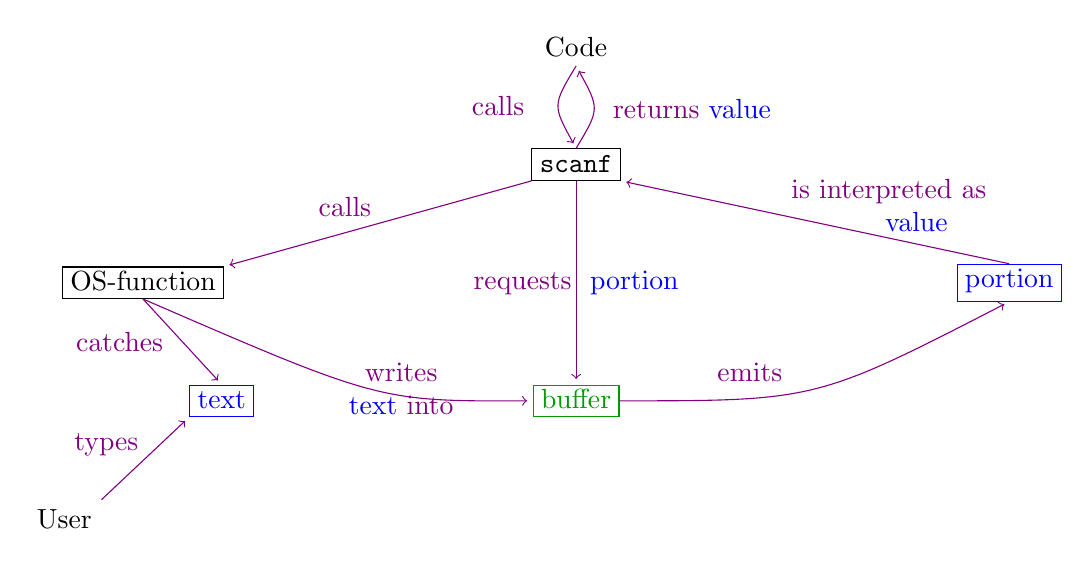
\begin{tikzpicture}
	[
		agent/.style={minimum width=1mm, text height=2mm, draw=black, inner sep=1mm},
		data/.style={minimum width=1mm, text height=2mm, draw=blue, inner sep=1mm},
		memory/.style={minimum width=1mm, text height=2mm, draw=green!60!black, inner sep=1mm},
		action/.style={draw=violet,shorten >=2pt,->}
	]
  
	\node (code)    at (6.5, 8.0) {Code};
	\node (scanf)   at (6.5, 6.5) [agent] {\texttt{scanf}};
	\node (buffer)  at (6.5, 3.5) [memory] {\color{green!60!black} buffer};

	\node (osfunc)  at (1.0, 5.0) [agent] {OS-function};
	\node (text)    at (2.0, 3.5) [data] {\color{blue} text};
	\node (user)    at (0.0, 2.0) {User};

	\node (portion) at (12.0, 5.0) [data] {\color{blue} portion};

	\draw [action] (code.south) 
		.. controls +(-0.3, -0.5) ..
		node [text width=2.2cm, midway, align=left] 
			{\color{violet} calls} 
		(scanf.north);
	\draw [action] (scanf.north) 
		.. controls +(+0.3, +0.5) ..
		node [text width=4.5cm, midway, align=right] 
			{\color{violet} \phantom{aa}returns \color{blue}value} 
		(code.south);
	
	\draw [action] (scanf.south west) 
		-- 
		node [text width=1.5cm, midway] 
			{\color{violet} calls \\ \phantom{a}} 
		(osfunc.north east);
	
	\draw [action] (osfunc.south) 
		-- 
		node [text width=2.7cm, midway] 
			{\color{violet} catches} 
		(text.north);
	\draw [action] (user.north east) 
		-- 
		node [text width=1.8cm, midway] 
			{\color{violet} types\\ \phantom{a}}
		(text.south west);
	
	\draw [action] (osfunc.south) 
		.. controls +(3.0, -1.3) ..
		node [text width=3.0cm, midway, align=center] 
			{\phantom{aaaa} \color{violet} writes \\
			 \phantom{aaaa} {\color{blue} text} into
			} 
		(buffer.west);
	
	\draw [action] (scanf.south) 
		--
		node [text width=5cm, midway, align=center] 
			{\color{violet} requests~~\color{blue}portion} 
		(buffer.north);
	
	\draw [action] (buffer.east) 
		.. controls +(2.5, 0.0) ..
		node [text width=2.5cm, midway, align=left] 
			{\color{violet} emits \\ \phantom{a}} 
		(portion.south);
	\draw [action] (portion.north) 
		-- 
		node [text width=5.5cm, midway, align=center] 
			{\phantom{aaaaaaaaaa} \color{violet} is interpreted as \\ 
			 \phantom{aaaaaaaaaaaaaa} \color{blue} value \\
			 \phantom{a}
			 }
		(scanf.south east);
\end{tikzpicture}
\end{center}
\captionof{figure}{\texttt{scanf} action flowchart} \label{fig:scanfActionFlowchart}
\end{defbox}

This means that, when calling \texttt{scanf}, there might be leftover text from an earlier keybord interaction with the user. When this is the case, the OS will not wait for the user to type any text, but rather forward the remaining content of the buffer (or even again only a portion thereof). Knowing this, we can understand why the following code behaves as it does:

\begin{tcbraster}[raster columns=2,
                  raster equal height,
                  nobeforeafter,
                  raster column skip=0.2cm]
\begin{codebox}[keyboardBuffer.c]
\begin{minted}[linenos]{c}
#include <stdio.h>

int main () {
    int i;
    double d;

    scanf("%d", &i);
    scanf("%lf", &d);

    printf("%d and %lf\n", i, d);
}
\end{minted}
\captionof{code}{Remaining Text in the keyboard buffer}
\end{codebox}
%
\begin{cmdbox}[Possible Output: keyboardBuffer.c]
12.3 \\
12 and 0.300000
\end{cmdbox}
\end{tcbraster}

\begin{hintbox}[Use expressive names]
Having trouble with the above example? There's a \texttt{d} in the format string, meaning \inC{int}eger and a variable \texttt{d} which is a \inC{double}. This is certainly confusing.

I mentioned before that names should be as expressive as possible. My experience is that a good deal of students disregard this advice until they run into problems. So, if you belong to that crowd: here you are, home made problems. You're welcome.

It is often said that good code should read like prose. This certainly is sometimes hard to achieve, especially here, where we often regard code that is only to illustrate a concept and does not come with any context attached to it; but we should always at least try to make an effort with our variables. So, maybe the above example becomes clearer in this form:

\begin{codebox}[keyboardBuffer.c]
\begin{minted}[linenos]{c}
#include <stdio.h>

int main () {
    int preDecimalDot;
    double postDecimalDot;

    scanf("%d", &preDecimalDot);
    scanf("%lf", &postDecimalDot);

    printf("%d and %lf\n", preDecimalDot, postDecimalDot);
}
\end{minted}
\captionof{code}{Remaining Text in the keyboard buffer (better variable names)}
\end{codebox}
\end{hintbox}

Let us also look at this slightly more involved example:

\begin{codebox}[enterExpression.c]
\begin{minted}[linenos]{c}
#include <stdio.h>

int main () {
    char operator = 0;
    double operand1 = -1, operand2 = -1;

    printf("Please enter a simple expression (like 2+2): ");
    scanf("%lf", &operand1);
    scanf("%c" , &operator);
    scanf("%lf", &operand2);

    printf("%lf %c %lf\n", operand1, operator, operand2);
}
\end{minted}
\captionof{code}{Reading two numbes and an operator with \texttt{scanf}} \label{code:scanf_lfclf}
\end{codebox}
(Remember, that the type \inC{char} stores one charcter; essentially one letter worth of information. Characters are internally stored as numbers between 0 and 255 and \enquote{translated} by means of the ASCII table.)

Let's first assume, our user knows neither about the keyboard buffer nor what our code looks like internally. When running the code, they are very likely to follow our prompt verbatim:
\begin{cmdbox}[Possible Output: enterExpression.c]
Please enter a simple expression (like 2+2): 2+2 \\
2.000000 + 2.000000
\end{cmdbox}
Looks good. We still want to take the time to understand what is happening here in detail:

Although there are three \texttt{scanf} commands, the operating system requests text only once. We understand now, why this is so. When we hit line 8, there is nothing in the keyboard buffer. Consequently, the operating system waits till the user presses enter and puts everything up to that point into the keyboard buffer. Then, the portion of the entered text that meets the format string \texttt{\%lf} is interpreted as double. Since the symbol \texttt{+} cannot appear in the middle of a floating point number, interpretation stops there; only the first \texttt{2} is interpreted. Thereafter, line 9 is executed. Since the keyboard buffer is still not empty (it still contains \texttt{+2}), the operating system does not wait for user input; instead, the next portion is forwarded to \texttt{scanf}. Since only a single character was requested (\texttt{\%c}), \texttt{scanf} receives \texttt{+}. Finally, by line 10 we have a last \texttt{2} in the buffer, which eventually gets converted into a \inC{double} and stored in \texttt{operand2}.

Now, what if the user likes seperating numbers from operators?
\begin{cmdbox}[Possible Output: enterExpression.c]
\begin{minted}{text}
Please enter a simple expression (like 2+2): 2 + 2
2.000000   -1.000000
\end{minted}
\end{cmdbox}

Like before, the \texttt{scanf} in line 8 stops after the first \texttt{2}. However, this time, we don't get to the plus sign, because before that there's a whitespace (that cannot be part of a number, either). Consequently, line 9 takes that whitespace out of the queue and leaves \texttt{+ 2} in the buffer. When we arrive at line 10, we find this situation: a number may begin with a plus sign, but a whitespace still doesn't fit the bill. \texttt{+} at its own is not a number, so interpretation fails. The whitespaces is put back into the buffer (as it can't be part of a number), but the plus sign was already accepted as valid. So in the keyboard buffer we now find a whitespace followed by a \texttt{2}.

One last execution example. We as coders and testers know that there actually are three calls to \texttt{scanf}. So what if we hit enter after each element of the input (\texttt{2}, enter, \texttt{+}, enter, \texttt{2}, enter)?

\begin{cmdbox}[Possible Output: enterExpression.c]
\begin{minted}{text}
Please enter a simple expression (like 2+2): 2
+ 
2.000000 
 -1.000000
\end{minted}
\end{cmdbox}

We don't even get the chance to enter a second number. The reason behind this is that the return key is written into the keyboard buffer as well. So, executing line 8 unfolds as following: The user (by means of the OS function) writes "\texttt{2}, enter" into the keyboard buffer. \texttt{scanf} then takes out the \texttt{2}, but leaves the enter in the line break. The \texttt{scanf} in line 9 reads this very character and thus leaves an empty keyboard buffer. Finally, in line 10 we are ready to take new input from the keyboard. As users we were unaware that we skipped a part of the questionaire and enter a \texttt{+}, which is an acceptable starting character for a number (and hence taken out of the keyboard buffer) but does not encode a complete number, which is why the interpretation step fails. We end up with this state of memory:
{
\newcolumntype{N}{>{\ttfamily\centering\arraybackslash} p{.25\linewidth}}
\newcolumntype{R}{>{\ttfamily\centering\arraybackslash} p{.15\linewidth}}
\begin{center}
\rowcolors{1}{tabhighlight}{white}
\begin{tabularx}
	{.45\linewidth}
	{NR}
\toprule[1.5pt]

    \textrm{\textbf{Variable}} & 
    \textrm{\textbf{Value}}  
\tabcrlf
    operand1   & 2  \\
    operator   & \textbackslash n \textrm{(newline)}  \\
    operand2   & -1  \\

\bottomrule[1.5pt]
\end{tabularx}
\end{center}
}

So... If line breaks are written into the keyboard buffer, too, how does example \ref{code:scanfSimple} work out? There we asked for two numbers in a row and got exactly what we asked for, with no issues. The reason for this is that the subroutine for interpreting numbers is written such that it ignores all whitespaces, tabulators or line breaks. When you read input with \texttt{\%d} or \texttt{\%lf}, leading characters belonging to this group are taken out of the buffer and simply discarded.

We can activate the same behaviour for when we read characters: to do so, we simply put a whitespace in our format string before the \texttt{\%c}. This then translates to \enquote{read a single character, but ignore all whitespaces, tabulators or line breaks}. Knowing this we can get around all of the problems we just discussed by improving on code \ref{code:scanf_lfclf}:
\begin{codebox}[enterExpressionImproved.c]
\begin{minted}[linenos]{c}
#include <stdio.h>

int main () {
    char operator = 0;
    double operand1 = -1, operand2 = -1;

    printf("Please enter a simple expression (like 2+2): ");
    scanf("%lf", &operand1);
    scanf(" %c", &operator);
    scanf("%lf", &operand2);

    printf("%lf %c %lf\n", operand1, operator, operand2);
}
\end{minted}
\captionof{code}{Reading two numbes and an operator with \texttt{scanf} (more stable version)} \label{code:scanf_lfclf_stable}
\end{codebox}

It takes a keen eye to spot the difference: codes \ref{code:scanf_lfclf} and \ref{code:scanf_lfclf_stable} are almost identical except for a single extra whitespace in the format string in line 9. And with this simple trick...
\begin{cmdbox}[Possible Output: enterExpressionImproved.c]
\begin{minted}{text}
Please enter a simple expression (like 2+2): 2    +  2
2.000000 + 2.000000
\end{minted}
\end{cmdbox}
... user input is no longer a problem.

\begin{hintbox}[Test your code independent from user input]
If this chapter so far has taught you anything then that user input is a finnicky thing. Not only could it be that a user enters wrong or even nonsensical values; it isn't even always easy to see what constitutes a nonsensical value. This makes develloping algorithms difficult, as it's not immediately clear whether an unexpected result comes from a problem with the code itself or with the user input.

For that reason, it is best to implement user input only at the very end of the devellopment process. Where values are needed, we can simply hard code the values of our variables and leave the \texttt{scanf} lines commented out. Only when we are sure that the algorithm itself does what we want it to do, we turn on interactivity.

Code under devellopment might look like...
\begin{codebox}[someAlgorithm-devellopment.c]
\begin{minted}[linenos]{c}
#include <stdio.h>

int main () {
    int input = 1337;        // reasonable value as stand-in for user input
    // scanf("%d", &input)   // commented out for testing
    
    /* ... Your code under test here ... */
}
\end{minted}
\captionof{code}{Code under devellopment -- \texttt{scanf} commented out}
\end{codebox}
\end{hintbox}
%
\begin{hintbox}[]
... while the final version will be like:
\vspace{6pt}

\begin{codebox}[someAlgorithm-productive.c]
\begin{minted}[linenos]{c}
#include <stdio.h>

int main () {
    int input = 0;        // default value if the user enters BS
    scanf("%d", &input)
    
    /* ... Your well tested code here ... */
}
\end{minted}
\captionof{code}{Productive code -- \texttt{scanf} active}
\end{codebox}
\end{hintbox}

\begin{defbox}[Main Takeaways for this section]
To put the results of our deep dive in this section into a nutshell:
\begin{itemize}
\item \texttt{scanf} delegates text input to the operating sytem (OS) and only interprets values from a keyboard buffer.
\item It takes out only so much text from the keyboard buffer as makes sense given the current format string.
\item If there is leftover text in the keyboard buffer, it is interpreted directly. The user cannot enter any text in this case.
\item Even the enter key leaves a line break character in the keyboard buffer.
\item When you want to ignore separating characters like whitespaces in the user input, add a whitespace in the format string before the placeholder (before the percent sign).
\end{itemize}
\end{defbox}

\subsection{Reading Multiple Values in Sequence} \label{sec:ScanfMultiValues}
It should be noted that a \texttt{scanf} format string can hold more than one placeholder (\ie a percent sign \% followed by a type symbol like \texttt{d} or \texttt{lf}). This then has the same effect as several \texttt{scanf} commands with a single placeholder in sequence. The addresses to which the values are written are simply provided as a comma separated list, as with \texttt{printf}. Thus, the lines 8 through 10 from code \ref{code:scanf_lfclf_stable} can be condensed into the single line:
\mint{c}{scanf("%lf %c%lf", &operand1, &operator, &operand2);}
This saves some typing, but, however, comes at the cost of clarity and user friendliness.

In section \ref{sec:scanf_keyboardBuffer} we discussed that a whitespace in the format string does make a difference. By consequence, the elements of a multi placeholder \texttt{scanf} format string are very dense and hard to grasp. This lends itself to all sorts of mistakes like type mismatches (cf. section \ref{sec:scanfMistakes}). A \texttt{scanf} line allows for many degrees of freedom: there are a multitude of variations that differ by only a single character but give a very different behaviour. Limiting the length of a \texttt{scanf} line reduces the amount of detail we as human programmers have to handle in our heads and reducing mental load is a good way to prevent making mistakes.

Secondly, users of our program need to be guided on how to use it. If you start a program and you see nothing but a blinking cursor, you might infer that the program has crashed, when in reality in only runs a \texttt{scanf} command and waits for you to enter a value. So it's best to preface each \texttt{scanf} with a \texttt{printf} that tells the user what to enter. Of course you could write a prompt like \emph{Please enter three numbers}. But how to separate these three values? For a non-expert, options like pressing enter after each value (valid) or separating them with a comma (invalid) might come to mind. Instead of typing a lengthy human explanation how many values in which form the program expects, it's better to type slightly more commands and limit the complexity for the user. Because they, too, are humans, and will make more mistakes the more complex the task demanded from them becomes.

\subsection{Common Mistakes} \label{sec:scanfMistakes}
There are a number of mistakes that even experienced coders make from time to time. It is easy to write C-Code that does compile but has an unintended effect. Here, I want to discuss some of the most common mistakes one can make when using \texttt{scanf}.

\subsubsection{Forgetting the Ampersand}
You remember that \texttt{scanf} needs an \emph{address} to write the interpreted value to. You also remember that you get the address of a variable with the ampersand operator (\texttt{\&}).  What would happen, if you forgot that operator?

In a word, the result is \emph{unpredictable}. We also say, \emph{using an invalid address gives undetermined behaviour}. If you forget to use the address operator \texttt{\&}, whatever value was stored in the variable is interpreted as an address. So essentially, you get a random address to which you write. Who can say what this memory location is being used for?

There are three possible scenarios:
\begin{itemize}
\item The random address points to \emph{unused memory}. You write the user input into a random cell that nobody knows about -- the result is \enquote{forgotten}.
	Your target variable is not updated, but the return value from \texttt{scanf} indicates that a value was correctly read.
\item The random address points to \emph{used memory}. You overwrite the value of some variable, but not the one you wanted to change, which remains untouched.
\item The random address points to \emph{forbidden memory}. There are memory sections that can only be changed by certain programs, to ensure a stable system. The operating system
	\emph{watches} each program's activities. If one of them tries to access a forbidden section (\eg the section where the operating system itself resides), it refuses the access and
	shuts the program down. You will see an error message about a \emph{segmentation fault} (often abbreviated to segfault), which is the formal terminus for accessing forbidden memory.\\
	A variation thereof is \emph{stack smashing}. The difference between a segfault and stack smashing is subtle, and understanding it won't help us much.
	Simply remember that both mean \emph{access to forbidden memory}.\\
	Segfaults and Stack Smashing are the most likely outcome of forgetting the ampersand.
\end{itemize}

It actually is difficult to synthesize the first two of the above scenarios; however, we can reliably reproduce \emph{segfaults} and \emph{stack smashing}.

\begin{warnbox}[segfault.c, leftupper=7mm]
\begin{minted}[linenos]{c}
#include <stdio.h>

int main () {
    int value = 0;
    
    printf("Enter a value: "); 
    scanf("%d", value);
    
    printf("%d\n", value);
}
\end{minted}
\captionof{code}{Causing a segfault with \texttt{scanf}}
\end{warnbox}

Executing this program simply ends in a crash:
\begin{cmdbox}[Output: segfault.c]
\begin{minted}{text}
Enter a value: 0
Segmentation fault (core dumped)
\end{minted}
\end{cmdbox}

Note that the compiler already warns us that we've made a mistake:
\begin{cmdbox}[Compiler Warnings: segfault.c]
\begin{minted}{text}
$ gcc -Wall -Wextra -Wpedantic 
    segfault.c -o segfault
segfault.c: In function ‘main’:
segfault.c:7:13: warning: format ‘%d’ expects argument of type ‘int *’,
    but  argument 2 has type ‘int’ [-Wformat=]
    7 |     scanf("%d", value);
      |            ~^   ~~~~~
      |             |   |
      |             |   int
      |             int *
\end{minted}
\end{cmdbox}
%$

Stack smashing can only occur when the number is an \emph{almonst valid} address, \ie very close to a point in memory that we are allowed to access. Modern computers use 64bit addresses, while an \inC{int} is only a 32bit variable. Hence, the example below uses the data type \inC{long long int}, together with the format string \texttt{\%lld}, which stands for this data type. In its core, the example below has the same structure as the one above. Only the initial value is such an \emph{almost valid} address.

\begin{warnbox}[stackSmashing.c, leftupper=7mm]
\begin{minted}[linenos]{c}
#include <stdio.h>

int main () {
    long long int value = &value + 1;
    
    printf("Enter a value: ");
    scanf("%lld", value);
    
    printf("%lld\n", value);
}
\end{minted}
\captionof{code}{Causing stack smashing with \texttt{scanf}}
\end{warnbox}

Again, the compiler tries to warn us:
\begin{cmdbox}[Compiler warnings: stackSmashing.c]
\begin{minted}{text}
$ gcc -Wall -Wextra -Wpedantic stackSmashing.c -o stackSmashing
stackSmashing.c: In function ‘main’:
stackSmashing.c:4:27: warning: initialization of ‘long long int’ from 
    ‘long long int *’ makes integer  from pointer without a cast 
    [-Wint-conversion]
    4 |     long long int value = &value + 1;
      |                           ^
stackSmashing.c:7:15: warning: format ‘%lld’ expects argument of type 
    ‘long long int *’, but argument 2 has type ‘long long int’ [-Wformat=]
    7 |     scanf("%lld", value);
      |            ~~~^   ~~~~~
      |               |   |
      |               |   long long int
      |               long long int *
\end{minted}
\end{cmdbox}
%$

Executing the code, we get what we deserve:
\begin{cmdbox}[Output: stackSmashing.c]
\begin{minted}{text}
Enter a value: 0
140732161677208
*** stack smashing detected ***: terminated
Aborted (core dumped)
\end{minted}
\end{cmdbox}

\subsubsection{Using the wrong Format String Elements}
As far as the computer is concerned, the \texttt{scanf} command means the following: take some text from the keyboard, convert it into a bitpattern according to rules set out in a format string, and write them to some specified address. This set of instructions does not involve checking whether the bitpattern makes any sense at the target address\footnote{because such a check would not be possible}. If you tell the computer to write a floating point value to an integer address, it will comply -- only that the result is nonsensical (at best). Let's regard two examples:
\begin{tcbraster}[raster columns=2,
                  raster equal height,
                  nobeforeafter,
                  raster column skip=0.2cm]
\begin{warnbox}[typeMismatch.c, leftupper=7mm]
\begin{minted}[linenos]{c}
#include <stdio.h>

int main () {
    double value = 0.0;
    
    printf("Enter a value: "); 
    scanf("%d", &value);
    
    printf("%lf\n", value);
}
\end{minted}
\captionof{code}{Type mismatch with \texttt{scanf}}
\end{warnbox}
%
\begin{cmdbox}[Output: typeMismatch.c]
\begin{minted}{text}
$ gcc -Wall -Wextra -Wpedantic 
    typeMismatch.c -o typeMismatch
$ ./typeMismatch
typeMismatch.c: In function ‘main’:
typeMismatch.c:7:13: warning: format 
    ‘%d’ expects argument of type 
    ‘int *’, but argument 2 has type 
    ‘double *’ [-Wformat=]
    7 |     scanf("%d", &value);
      |            ~^   ~~~~~~
      |             |   |
      |             |   double *
      |             int *
      |            %le
Enter a value: 2.718 
0.000000
\end{minted}
\end{cmdbox}
\end{tcbraster}
Here we told the computer to read an integer (\texttt{\%d}) to a \inC{double} slot. As predicted, the result (\texttt{0.0}) has nothing to do with what we entered (\texttt{2.718}). At least, our trusted friend the compiler warns us again of this mistake.

A somewhat worse version is this:
\begin{tcbraster}[raster columns=2,
                  raster equal height,
                  nobeforeafter,
                  raster column skip=0.2cm]
\begin{warnbox}[bleeding.c, leftupper=7mm]
\begin{minted}[linenos]{c}
#include <stdio.h>

int main () {
    int val1 = -1, val2 = -1;

    printf("Enter a value: ");
    scanf("%lf", &val1);

    printf("value 1 = %d\n", val1);
    printf("value 2 = %d\n", val2);
}
\end{minted}
\captionof{code}{bleeding with \texttt{scanf}}
\end{warnbox}
%
\begin{cmdbox}[Output: bleeding.c]
\begin{minted}{text}
$ gcc -Wall -Wextra -Wpedantic 
    bleeding.c -o bleeding
$ ./bleeding
bleeding.c: In function ‘main’:
bleeding.c:7:14: warning: format 
    ‘%lf’ expects argument of type 
    ‘double *’, but argument 2 has 
    type ‘int *’ [-Wformat=]
    7 |     scanf("%lf", &val1);
      |            ~~^   ~~~~~
      |              |   |
      |              |   int *
      |              double *
      |            %d
Enter a value: 1
value 1 = 0
value 2 = 1072693248
\end{minted}
\end{cmdbox}
\end{tcbraster}

Not only did we not get what we expected for \texttt{val1}; the \texttt{scanf} command also destroyed the information stored in \texttt{val2}!

To understand this, you have to know that \texttt{val1} and \texttt{val2} are (in this example) arranged in memory such they are right next to each other. Each of them is a variable of type \inC{int}, which means it takes up 32 bit or 4 Byte worth of memory. The \enquote{write-command} in \texttt{scanf} tells the computer to write a value of type \inC{double}, which is 64 bits or \emph{eight} bytes: we write over the confines of one \enquote{memory compartment} (the variable \texttt{val1}) and \enquote{bleed} into the next compartment (the variable \texttt{val1}).

\begin{defbox}[Memory Picture]
\begin{center}
\begin{tikzpicture}
  [
    minicell/.style={text width= 3mm, text height=2mm, draw=black, inner sep=1mm},
    widecell/.style={text width=18mm, text height=4mm, draw=black, inner sep=1mm},
    ld/.style={draw=blue,shorten >=2pt,->}
  ]
  
  \node (c0) at (0.0, 8) [minicell] {};
  \node (c1) at (0.5, 8) [minicell] {};
  \node (c2) at (1.0, 8) [minicell] {};
  \node (c3) at (1.5, 8) [minicell] {};
  \node (p0) [below=0mm of c0] {\tiny \color{blue} 0x27fb};
  \node (p1) [below=2mm of c1] {\tiny 0x27fc};
  \node (p2) [below=0mm of c2] {\tiny 0x27fd};
  \node (p3) [below=2mm of c3] {\tiny 0x27fe};
  \node (C0) at (0.75, 8.5) [widecell, align=center] {\texttt{val1}};
  
  \node (c4) at (2.0, 8) [minicell] {};
  \node (c5) at (2.5, 8) [minicell] {};
  \node (c6) at (3.0, 8) [minicell] {};
  \node (c7) at (3.5, 8) [minicell] {};
  \node (p4) [below=0mm of c4] {\tiny 0x27ff};
  \node (p5) [below=2mm of c5] {\tiny 0x2800};
  \node (p6) [below=0mm of c6] {\tiny 0x2801};
  \node (p7) [below=2mm of c7] {\tiny 0x2802};
  \node (C1) at (2.75, 8.5) [widecell, align=center] {\texttt{val2}};
  
  \node (c8) at (4.0, 8) [minicell] {};
  \node (c9) at (4.5, 8) [minicell] {};
  \node (cA) at (5.0, 8) [minicell] {};
  \node (cB) at (5.5, 8) [minicell] {};
  \node (p8) [below=0mm of c8] {\tiny 0x2803};
  \node (p9) [below=2mm of c9] {\tiny 0x2804};
  \node (pA) [below=0mm of cA] {\tiny 0x2805};
  \node (pB) [below=2mm of cB] {\tiny 0x2806};
  \node (C2) at (4.75, 8.5) [widecell] {...};
  
  \node (cC) at (6.0,8) [minicell] {};
  \node (cD) at (6.5,8) [minicell] {};
  \node (cE) at (7.0,8) [minicell] {};
  \node (cF) at (7.5,8) [minicell] {};
  \node (pC) [below=0mm of cC] {\tiny 0x2807};
  \node (pD) [below=2mm of cD] {\tiny 0x2808};
  \node (pE) [below=0mm of cE] {\tiny 0x2809};
  \node (pF) [below=2mm of cF] {\tiny 0x280A};
  \node (C2) at (6.75, 8.5) [widecell] {...};  

  \node (lblAddress)   at (-2, 7.5) {address of \texttt{val1}};
  \node (lblCells)     at (-2, 8.0) {memory cells};
  \node (lblCompounds) at (-2, 8.5) {variables};
  
  \draw [ld] (lblAddress.east) .. controls +(0.3,0) .. (p0.west);
  \draw [
	    thick,
	    decoration={
	        brace,
	        mirror,
	        raise=0.8cm
	    },
	    decorate
	] (c0.west) -- (c7.east) 
node [pos=0.5,anchor=south,yshift=-1.5cm] {eight bytes for a \texttt{double} value}; 
\end{tikzpicture}
\end{center}
\captionof{figure}{Bleeding}
\end{defbox}

\begin{hintbox}[Double-check your pointer assignments]
As you've seen, not only can you get nonsensical data if you mix up the format strings and the variables that are written with these format strings; you can also destroy other values. As you can imagine, this makes debugging exceedingly difficult (try finding the point in the code that changes \texttt{val2}, if nothing in it seems to even touch it). It is therefore of utmost importance that you are always aware of the data types of the values that you want to write and the means by which you do so. This holds particularly for working with pointers.
\end{hintbox}

\subsubsection{Non-Placeholder Characters in the Format String}
When typing a \texttt{printf} format string, we pretty much always put a line break (\texttt{\textbackslash n}) at its end. It almost becomes an automatism. It is no surprise thus that, in my time as a teacher, I've seen several students putting the same sequence, and I can't blame them for their mistake\footnote{which is infuriatingly hard to spot.}. So, again, let's consider an example and see what happens if we compile and run it:

\begin{tcbraster}[raster columns=2,
                  raster equal height,
                  nobeforeafter,
                  raster column skip=0.2cm]
\begin{warnbox}[linebreakScanf.c, leftupper=7mm]
\begin{minted}[linenos]{c}
#include <stdio.h>

int main () {
    int val1 = -1, val2 = -1;

    printf("Enter a value: ");
    scanf("%d\n", &val1);

    printf("Enter another value: ");
    scanf("%d\n", &val2);

    printf("value 1 = %d\n", val1);
    printf("value 2 = %d\n", val2);
}
\end{minted}
\captionof{code}{Line break in format string of \texttt{scanf}}
\end{warnbox}
%
\begin{cmdbox}[Output: linebreakScanf.c]
\begin{minted}{text}
Enter a value: 1
2
Enter another value: 3
value 1 = 1
value 2 = 2
\end{minted}
\end{cmdbox}
\end{tcbraster}

At first, everything looks okay -- no compiler warnings. We can execute and run our code, and up to line 6 everything looks normal. Then we hit the \texttt{scanf} statement, which allows us to enter a value (in this case \texttt{1}). Strangely, though, after that we are not prompted to enter another value (line 9). Instead, the terminal allows us to directly enter \texttt{2}. Only then, line 9 is executed, \ie we are prompted to enter another value. However, when we get to lines 12 and 13, we see that this input has seemingly been ignored, and instead, the value \texttt{2} got into \texttt{val2}, even before line 10 (the only line writing to the address of \texttt{val2}) was exectued.

How is this possible? Of course, this has again to do with the keyboard buffer (cf. section \ref{sec:scanf_keyboardBuffer}). The line break in the format string (\texttt{\textbackslash n}) is understood as \enquote{put one value on hold}. That means, text is read from the keyboard but not interpreted at all. Rather than that, it is simply written to the keyboard buffer, ready to be picked up by a subsequent \texttt{scanf} call\footnote{There are some more fishy details here, but it's best to simply put no line breaks or non-placeholders into a format string at all. The sole exception, of course, are whitespaces.}.


\section{Type Casting}
So far we have a pretty good idea how data looks like in memory and how to get it there. We can also do computations and print the results on screen. For these operations to work properly, it is important to use the correct data types. As you can imagine, this can bring us in situations where we have information in one format, but need it in another. \emph{Type casting} is the operation that allows just that.

\subsection{Explicit Type Casts}
To do type casting, we need two things: a value (or expression) to cast into a new format, and the new format itself. The syntax for issuing a type cast is barely more than naming these two elements:
\begin{codebox}[Syntax: Type Casting]
\inC{(dataType) expression}
\end{codebox}
In which \texttt{dataType} is any data type as we've encountered them in chapter \ref{chp:expressions}, \eg \inC{int} or \inC{double*}, and \texttt{expression} is anything that can be evaluated.

Let's look at an example:
\begin{codebox}[Example: typecast.c]
\begin{minted}[linenos]{c}
int main () {
    int    n = 7;
    double x = (double) n,
           y = (double) (2 + 4 * n);
}
\end{minted}
\captionof{code}{Typecasting}
\end{codebox}
Line 2 declares a \inC{int} variable \texttt{n} and assigns it the value \inC{7}. In line 3 we declare a \inC{double} variable \texttt{x} and assign it the result of a typecast: we cast the value of \texttt{n} to \inC{double}, \ie we compute \inC{7.0} from \inC{7}. Line 3 shows that we can combine this with regular computations, too: we first evaluate \inC{2 + 4 * n} to \inC{30}, and then cast it to \inC{double}, which then gives \inC{30.0}.

Note that in line 4, parentheses around the expression are necessary, since type casting has very high operator precedence (\ie it is evaluated even before multiplication. See also table \ref{tab:OperatorPrecedence} in the appendix). If we forgot to put \inC{2 + 4 * n} in parentheses, the typecast would only apply to the first number. That means, we first convert \inC{2} to a \inC{double}, then the \inC{int} value of \inC{4 * n} is computed, and then the mixed type expression \inC{2.0 + 28} is resolved. You'll see in the next section how that turns out.

While a type cast will leave as much information intact as possible, you may loose information in the process. Casting a \inC{double} into an \inC{int} can obviously not retain the fractional part of the number. Instead, the number is \emph{truncated} (rounded towards zero; the fractional part is simply forgotten):

\begin{codebox}[Example: typecastPrecisionLoss.c]
\begin{minted}[linenos]{c}
int main () {
    double x = +7.9,
           y = -7.9;

    int a = (int) x,  // +7
        b = (int) y;  // -7
}
\end{minted}
\captionof{code}{Typecasting with loss of precision}
\end{codebox}

As you see, this is different from rounding. We will see in chapter \ref{chp:maths} how to implement rounding\footnote{Some forum posts recommend adding \texttt{0.5} to positive numbers or subtracting that value from negative values before typecasting. That certainly works, but I will show you a nicer, better legible way later on.}.

In a similar fashing, numbers that require more bits than the target type are truncated: Let's say we want to cast the \inC{int 257} to a \inC{char}. An \inC{int} can store 32 bits, so the value $257_{10} = 1~0000~0001_2$ with its nine bits fits snuggly into the provided space. A \inC{char} on the other hand only has space for eight bits. So anything to the left of the eighth bit is simply truncated. We get:

\begin{codebox}[Example: typecastOverflow.c]
\begin{minted}[linenos]{c}
int main () {
    char data = (char) 257; // data = 1
}
\end{minted}
\captionof{code}{Typecasting with overflow}
\end{codebox}

\subsection{Implicit Type Casts}
The C compiler tries to save you some typing by issuing some typecasts without you explicitly saying so. These implict type casts happen in two situations:
\begin{itemize}
\item Variable assignments
\item Mixed type expressions
\end{itemize}

Let's say, in your code you write a line like \inC{double x = 7;}. The value \inC{7} is an \inC{int} (there's no decimal point). Hence, implicitly, the value \inC{7} is cast to \inC{7.0} before the assignment. Of course, the same limitations to casting apply as in the explicit form: casting to an integer data type will truncate the fractional part, and casting to a smaller data type will truncate the highest significant bits.

In the case of mixed type expressions, the C compiler again tries to retain as much information as possible. The operands of an expression are implicitly cast to a common type that is wide enough (has enough bits of storage) to hold either operand, and to a floating point type if either of the operands is one. If you evaluate the expression \texttt{a + b}, where \texttt{a} and \texttt{b} are of different data types, then both of them will be cast to either the type of \texttt{a} or of \texttt{b} and follow this \enquote{hierarchy of promotions}:
\begin{center}
	\inC{char < short < int < long < long long < float < double < long double}
\end{center}

For example, ...
\begin{codebox}[Example: promotion.c]
\begin{minted}[linenos]{c}
int main () {
    double x = 8 / 5.0;
}
\end{minted}
\captionof{code}{Implicit type cast with promotion}
\end{codebox}

The value \inC{8} is of type \inC{int}, while \inC{5.0} is of type \inC{double}. To perform the division, \inC{8} is implicitly cast to the \inC{double} value \inC{8.0} before the division takes place.

\begin{plusbox}[Type Suffixes]
You remember that, to represent floating point numbers in memory, you can use the data types \inC{double}, \inC{float} or \inC{long double}. If a decimal number (anything that contains a decimal point) appears in the code, it will be interpreted as a \inC{double} value by default, while integers will be treated as \inC{int}s. To deviate from this default behaviour, a suffix can be added to the number: \inC{1.2f} will be converted to a \inC{float} value rather than a double. Similarly, other data types have their proper suffixes, too.

In the appendix you can find table \ref{tab:LiteralFormat} which lists all modifiers that can be added to a number literal. If a given type is not listed in this table, you'd need to explicitly typecast the literal, \eg \inC{(char)(7)}.
\end{plusbox}

In the previous example we've seen the expression \inC{(double) (2 + 4 * n)} and noted that, due to operator precedence, the second pair of parentheses is necessary. If we ommitted them, the explicit type cast would only apply to the \inC{2} while \inC{4 * n} remains an \inC{int} expression, making the entire expression mixed type. As we've seen before, the \inC{int} part is then promoted to a \inC{double}. So in principle, the final outcome is the same: the entire expression gets converted to \inC{double}. However, there are subtle differences: the computer has to do more work that way, and the result may accrue more rounding errors.

In the example with parentheses, the computer sees two units of work: evaluating one \inC{int} expression and converting the result to \inC{double}. In the case without parenthesis, however, the steps are: converting \inC{2} to \inC{double}, evaluating \inC{4 * n} as \inC{int}, converting the result to \inC{double}, and then adding the two \inC{double} values together. Further, a \inC{double} expression takes slightly longer to evaluate -- adding floating point numbers is slower than adding integers.

Floating point values \emph{always} come with a rounding error. It is small enough to give results that are good enough by far most of the time, but errors add up. Doing two conversions to \inC{double} means making the same error twice, so the result of \inC{(double)(2) + (double)(4 * n)} is\footnote{or rather \emph{can be} ... the details are a can of worms I don't want to open here.} twice as wrong.


\subsection{Type Casts with Pointers}
We know pointers to be special integers, representing the number of a memory cell, together with an attached rule how to read the data there. Essentially being numbers, we can type-cast them, too. This of course only affects the pointer, not the information pointed to. Another way of explaining a pointer type cast is: changing the rules for how to read memory content.

Let's look at an example:
\begin{codebox}[Example: pointerCast.c]
\begin{minted}[linenos]{c}
#include <stdio.h>

int main () {
    int   value = 259;
    int*  intPointer = &value;
    char* charPointer = (char*) intPointer;

    printf("direct access            : %d\n", value);
    printf("access via int pointer   : %d\n", *intPointer);
    printf("access via char pointer  : %d\n", *charPointer);

    *charPointer = 4;
    printf("direct access after write: %d\n", value);
}
\end{minted}
\captionof{code}{Typecast with a pointer} \label{code:typecastPointer}
\end{codebox}

\begin{cmdbox}[Output: pointerCast.c]
\begin{minted}{text}
direct access            : 259
access via int pointer   : 259
access via char pointer  : 3
direct access after write: 260
\end{minted}
\end{cmdbox}

To make sense of this, let's look under the hood:
\begin{defbox}[Memory Picture]
\begin{center}
\begin{tikzpicture}
  [
    minicell/.style={text width=18mm, text height=4mm, draw=black, inner sep=1mm},
    widecell/.style={text width=78mm, text height=4mm, draw=black, inner sep=1mm},
    ld/.style={draw=blue,shorten >=2pt,->}
  ]
  
  \node (C0) at (3.0, 8.5) [widecell, align=center] {259 = $0...0~0001~0000~0011_2$};
  \node (c0) at (0.0, 7.85) [minicell] {$0000\;0011_2$};
  \node (c1) at (2.0, 7.85) [minicell] {$0000\;0001_2$};
  \node (c2) at (4.0, 7.85) [minicell] {$0000\;0000_2$};
  \node (c3) at (6.0, 7.85) [minicell] {$0000\;0000_2$};
  \node (p0) [below=1mm of c0] {\tiny \color{blue} 0x27fb};
  \node (p1) [below=1mm of c1] {\tiny 0x27fc};
  \node (p2) [below=1mm of c2] {\tiny 0x27fd};
  \node (p3) [below=1mm of c3] {\tiny 0x27fe};

  \node (lblCompounds) at (-3.0, 8.5) {\inC{int value}};
  \node (lblCells)     at (-3.0, 7.8) {byte sized cells};
  \node (lblAddress)   at (-3.0, 7.1) {address of \texttt{value}};
  
  \draw [ld] (lblAddress.east) .. controls +(0.3,0) .. (p0.west);
\end{tikzpicture}
\end{center}
\captionof{figure}{Distribution of an integer across memory cells}
\end{defbox}

The variable \texttt{value} is of type \inC{int} and thus takes up 32 bits or four bytes of memory. Its initial value, the number \texttt{259} requires at least nine bits to represent; the rest is padded with zeros. So, in total four chunks of eight bits are taken up by the variable \texttt{value}.

An oddity of this distribution is that the cells are read \enquote{right to left}: the last eight bits form the first byte. The bits 0 through 7 of the value \texttt{259} are $0000~0011_2 = 3_{10}$ go into the first cell, while the bits 8 through 15 ($0000~0001_2 = 1_{10}$) go into the second cell, and so on.

When in line 6 we cast \texttt{pointer} from an \inC{int*} to a \inC{char*}, we are chaning the rules what to do with the address: we are no longer evaluating a group of four bytes, but only a single byte. Both, \texttt{intPointer} and \texttt{charPointer} store the same address, but access via \texttt{charPointer} (line 10) applies a narrower scope than access via \texttt{intPointer} (line 9).

Of course, these two views on the same block of memory can also be used for writing data. In line 12 we replace a single byte in memory by the value \inC{4}. This replaced byte is still part of the sequence that makes up \texttt{value}. By consequence, we should not be surprised to find that variable with a new value.

\begin{plusbox}[Endianness]
The fact that bytes are read from the right to the left is not an universal truth. It \emph{is} the standard on IA-32 and x86-64 processors, \ie Intel and ARM processors (among others) follow this rule, but there are other processor manufacturers, too\citationneeded[https://xkcd.com/993/].

The presented way of distributing numbers across memory cells is the \emph{little endian} way, so called because numbers \emph{start with the little end}. Its counterpart consequently would be big endian. (And, just to make things interesting, there are also mixed endian or middle endian processors out there...)

The word endian or endianness is actually inspired by Jonathan Swift's \emph{Gulliver's Travels}, where characters known as Lilliputians are divided into those breaking the shell of a boiled egg from the big end (Big-Endians) or from the little end (Little-Endians).

Knowing the endianness of a processor is usually not necessary in the day to day business of a programmer; however it is relevant once a program is required to communicate with other machines which may use a different processor architecture (and endianness).
\end{plusbox}

Casting a pointer to a different type to change part of the value of a variable is rarely ever\footnote{but not never} useful. The example above was, again, only meant to illustrate a concept. The main take-away from this section up to here is this: while type-casts with \enquote{normal} variables compute a new value (a different representation of the same information), casting pointers does in fact not create a new bitpattern: an address remains an address. Instead, the effect of a pointer type cast is changing the rule of interpretation applied to the bits at the stored address.

It should be noted that, for pointer casts, too, the implicit form is possible. In code \ref{code:typecastPointer}, we could in principle shorten line 6 to:
\mint{c}{char* charPointer = intPointer}
The program would work in exactly the same way as discussed above. The only difference is a compiler warning during compilation:
\begin{cmdbox}[Compiler Output: pointerCast.c]
\begin{minted}{text}
./pointerCast.c: In function ‘main’:
./pointerCast.c:6:25: warning: initialization of ‘char *’ from incompatible pointer 
    type ‘int *’ [-Wincompatible-pointer-types]
    6 |     char* charPointer = intPointer;
      |                         ^~~~~~~~~~
\end{minted}
\end{cmdbox}

The reason for this warning is that we usually don't want to mess around with the atoms of values. It is more likely to accidentally copy the wrong pointer into a variable, thereby forming a hard to locate bug in your code. If you actually need to typecast a pointer, it is best to be explicit about that\footnote{and maybe add a comment to tell a later reader \emph{why} you would need that}.

\subsubsection{Void Pointers}
If we've learned anything so far, then the fact that data types are very important for computers. Consequently, the C compiler is very strict: if a construct in the language requires a certain data type, the compiler will usually not be content if you provide anything but that data type. The warning you get from implicit pointer type casts would be one example for that.

However, there are situations where it actually does not matter what kind of information can be found behind some pointer. When you tell the computer to copy 2000 bytes from one address to another, it does not matter if these 2000 bytes encode 500 \inC{int}s or 250 \inC{double}s. Only the addresses themselves (and the number 2000) are important. For situations like this, a dedicated data type exists: the \inC{void*}. You can think of this as an address \emph{without} rules of interpretation. You cannot dereference a \inC{void*} because there is no data type \inC{void}\footnote{but there is the keyword \inC{void}, which we will get to know better in chapter \ref{chp:funcs}}.

%TODO does not participate in type checks:
\begin{codebox}[Example: voidPointer.c]
\begin{minted}[linenos]{c}
int main () {
    int   value = 259;
    int*  intPointer = &value;
    char* charPointer = intPointer;    // causes warning
    
    void* voidPointer = intPointer;    // does not cause warning
    int* otherPointer = voidPointer;   // does not cause warning either
}
\end{minted}
\captionof{code}{Implicit type casts with void pointers}
\end{codebox}

%TODO use with printf @ %p

\section{Bitwise Operations}

%TODO
% C4 becomes: casting, promotion, scanf, bit magic

% Exo: ask user for two int: number and bit ID; tell if set or not

% exo when doing cppref: write function that rounds with arbitrary precision, i.e. round_to_decimal_places(x, n)

% ----------------------------------

%\section{Bitweise Logik und Bit-Shifting} \label{sec:BitwiseOperator}
%Für Elektronik-Anwendungen ist es oft nötig, einzelne Schalter an- oder auszuschalten. Meist geschieht dies über eine Zustandsvariable, die an einen \emph{Port} (ein Anschluss, über den Daten fließen können) gesendet wird. Diese Zustandsvariable ist dann \idR eine Ganzzahl-Variable, in der jedes Bit für einen eigenen Schalter steht. Wir benötigen also Mittel, um einzelne Bits zu manipulieren.
%
%Dazu stehen uns die Operatoren \texttt{\~}, \texttt{\&}, \texttt{|}, \texttt{\^}, \texttt{<{}<} und \texttt{>{}>} zur Verfügung.
%
%Die \emph{bitweise Negation} (NOT, auch \emph{1er Komplement} genannt) \texttt{\~} kehrt jedes Bit um. Betrachten wir die vorzeichenlose 8-Bit-Zahl \texttt{42} (\texttt{00101010}). Das Ergebnis der Negation ist der Wert \texttt{213} (Binärzahl \texttt{11010101}). Als Code lässt sich das wie folgt umsetzen:
%\begin{codebox}[Beispiel: Bitweise Negation]
%\begin{minted}[linenos]{c}
%int main () {
%   unsigned char source = 42;
%   unsigned char result = ~source;
%}
%\end{minted}
%\end{codebox}
%
%Das \emph{bitweise und} (AND) \texttt{\&} vergleicht die Bits von zwei Werten und setzt das Bit im Ergebnis nur, wenn beide Bits in den Vergleichswerten gesetzt waren (\ie den Wert 1 hatten).
%
%Beim \emph{bitweisen oder} (OR) \texttt{|} werden ebenfalls die Bits von zwei Werten verglichen. Das entsprechende Bit im Ergebnis wird jedoch bereits gesetzt, wenn mindestens eines der Vergleichsbits gesetzt war.
%
%Das \emph{bitweise ausschließliche oder} (XOR) \texttt{\^} arbeitet genauso wie das OR, setzt das Ergebnis-Bit jedoch nur, wenn \emph{genau} eines der Vergleichsbits gesetzt war.
%
%All dies lässt sich in den folgenden Wahrheits-Tabellen ausdrücken:
%\begin{codebox}[Wahrheitstabellen: Bitweise Operatoren]
%\begin{minted}{text}
%     1 1 0 0   12       1 1 0 0   12       1 1 0 0   12
%     1 0 1 0   10       1 0 1 0   10       1 0 1 0   10
%     - AND -   --       -- OR -   --       - XOR -   --
%     1 0 0 0    8       1 1 1 0   14       0 1 1 0    6
%\end{minted}
%\end{codebox}
%
%Als Code lässt sich das wie folgt umsetzen:
%\begin{codebox}[Beispiel: Bitweise Operatoren]
%\begin{minted}[linenos]{c}
%int main () {
%   unsigned char lhs = 12, rhs = 10,
%                 and, or, xor;
%   and = lhs & rhs;    // =  8
%   or  = lhs | rhs;    // = 14
%   xor = lhs ^ rhs;    // =  6
%}
%\end{minted}
%\end{codebox}
%
%Die Negation benötigt nur ein \emph{Argument} (Wert, mit dem gearbeitet wird), und wird daher \emph{unärer Operator} genannt. Für AND, OR und XOR sind zwei Werte nötig, weswegen diese als \emph{binäre Operatoren} bezeichnet werden. Die Argumente können auch komplexe Ausdrücke sein, also Ergebnisse von Berechnungen:
%\begin{codebox}[Beispiel: Bitweise Operatoren]
%\begin{minted}[linenos]{c}
%int main () {
%   unsigned char result = ~(2 + 7 * (18 & 5));
%}
%\end{minted}
%\end{codebox}
%
%Bitmuster können als ganzes nach links oder rechts verschoben werden. Hierzu dienen die Operatoren \texttt{<{}<} und \texttt{>{}>}.
%\begin{codebox}[Beispiel: Bitweise Operatoren]
%\begin{minted}[linenos]{c}
%int main () {
%   unsigned char toLeft  = 170 << 1;
%   unsigned char toRight =  85 >> 1;
%}
%\end{minted}
%\end{codebox}
%Dies löst folgende Veränderung aus:
%\begin{codebox}[Bitshift nach links bzw. nach rechts um jeweils eine Stelle]
%\begin{minted}{text}
%     1 0 1 0 1 0 1 0   170       0 1 0 1 0 1 0 1    85
%     ----- << 1 ----   ---       ----- >> 1 ----   ---
%     0 1 0 1 0 1 0 0    84       0 0 1 0 1 0 1 0    42
%\end{minted}
%\end{codebox}
%Bei einem Bitshift nach links werden die Bits am rechten Ende des Bitmusters mit nullen aufgefüllt.
%%Stellen, die am linken Ende über die Registerbreite der aufnehmenden Variable hinaus verschoben werden, gehen verloren.
%Stellen, die über das linke Ende hinaus verschoben werden, gehen verloren.
%Alles eben gesagte gilt analog für den Bitshift nach rechts.
%
%\begin{hintbox}[Multiplikation mit Zweierpotenzen]
%Ein Bitshift um \texttt{n} Stellen nach links entspricht der Multiplikation mit der Zahl $2^{n}$.
%Ein Bitshift um \texttt{n} Stellen nach rechts entspricht der Division durch die Zahl $2^{n}$ (Bei Ergebnissen mit Nachkommastelle wird abgerundet). Bitshifts werden schneller durchgeführt als Multiplikationen mit \texttt{*}.
%
%Dies gilt nur für Ganzzahlen, nicht aber für Fließkommazahlen.
%\end{hintbox}
%

%\begin{hintbox}[Farben als Hexadezimal-Werte]
%In der Computertechnik werden Farben häufig mit \emph{Hex-Codes} beschrieben. Dies sind sechsstellige Kombinationen aus Ziffern und den Buchstaben A bis F. Tatsächlich sind diese Codes drei aneinander gereihte Hexadezimalzahlen. Diese beschreiben jeweils den Rot-, Grün- und Blau-Anteil einer Farbe. Der Dezimalwert 255 (bzw. die Hexadezimalzahl \texttt{0xFF}) beschreibt dabei \enquote{volle Intensität}, 0 (oder \texttt{0x00} dagegen sagt aus, von der Teilfarbe kommt kein Beitrag. Damit kann die Farbe Orange dann ausgedrückt werden als \texttt{0xFF7F00}: Volle Intensität Rot (\texttt{FF}), halbe Intensität Grün (\texttt{7F}) und Blau-Anteil 0 (\texttt{00}).
%
%Siehe auch \url{https://de.wikipedia.org/wiki/Additive_Farbmischung}
%\end{hintbox}
%
%\begin{hintbox}[Zweier-Potenzen in der Computerwelt]
%\emph{Alles} in der Computertechnik ist um Potenzen der Zahl 2 aufgebaut.
%%Wir finden 32-bit und 64-bit-Betriebssysteme, USB-Sticks mit 2, 4, 8 oder 16 GB, oder sogar Bildschirmauflösungen wie 1024x768 Pixel.
%Diese Zahlen kommen derartig häufig vor, dass sie von TechnikerInnen bereits als \enquote{runde Zahlen} wahrgenommen werden. So feierte beispielsweise Randall Munroe, Author des Webcomics \href{https://www.xkcd.com/}{xkcd} seinen eintausendsten Strip mit dieser Veröffentlichung:
%
%\begin{center}
%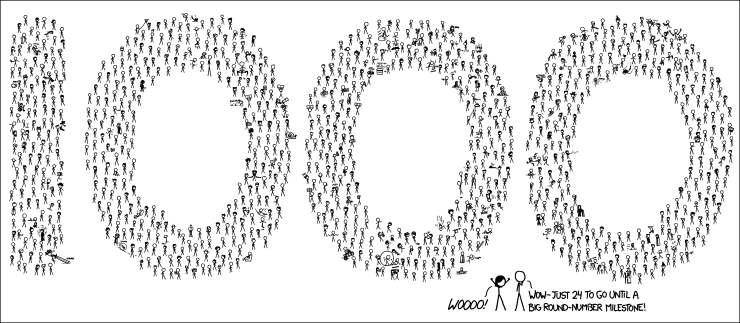
\includegraphics[width=.9\linewidth]{./gfx/xkcd-1000}
%\end{center}
%\captionof{figure}
%	[Dezimale und binäre runde Zahlen]
%	{Dezimale und binäre runde Zahlen. Quelle: \url{https://www.xkcd.com/1000/}}
%\end{hintbox}
